% Documento à parte: a árvore das combinações de testes, em um PDF próprio, com as
% definições de que ela precisa (formato, configurações e pares (N, f_c)).
% Compilar nesta pasta: pdflatex arvore_testes_documento.tex
% A figura vem de rascunho_arvore_testes.tex (a mesma que entra no TCC). As tabelas
% repetem a Tabela tab:paineis e a Tabela tab:n-condicao do texto
% (RESULTADOS/setup_simulacao.tex) e params.py (ALL_PANELS, M1_Driver.test_conditions).
\documentclass[11pt]{article}
\usepackage[utf8]{inputenc}
\usepackage[T1]{fontenc}
\usepackage[brazil]{babel}
\usepackage[a4paper, landscape, margin=0.9cm]{geometry}
\usepackage{amsmath, amssymb}
\usepackage{forest}
\usepackage{array}
\usepackage{graphicx}
\usepackage{xcolor}
\usepackage[normalem]{ulem}
% Edições de 2026-10-22: texto novo em vermelho; texto que saiu, riscado
\newcommand{\novo}[1]{\textcolor{red}{#1}}
\newcommand{\velho}[1]{\textcolor{red}{\sout{#1}}}
% \legend vem do abntex2 no TCC; aqui, só uma linha de texto abaixo da figura
\providecommand{\legend}[1]{\par\smallskip{\footnotesize #1}}
\pagestyle{empty}
% Fonte das caixas: no TCC, \scriptsize (padrão da figura); aqui, maior, para ocupar a página
\newcommand{\arvorefonte}{\small}
% Na figura do TCC, a legenda remete às tabelas do texto; aqui, às tabelas abaixo
\newcommand{\arvoredefinicoes}{as configurações e os pares $(N, f_c)$ estão nas tabelas da
página seguinte}

\begin{document}
% =====================================================================
% RASCUNHO -- árvore das combinações de testes, de cima para baixo: a raiz
% (os canais) no topo e cada teste feito como uma folha na última linha.
% ---------------------------------------------------------------------
% Para usar no texto: \input{chapters/tabelas/rascunho_arvore_testes}
% Precisa de \usepackage{forest} no preâmbulo. É larga: no TCC, usar
% em página deitada (pacote pdflscape) ou com \resizebox{\textwidth}{!}{...}.
% Documento à parte, só com a figura: chapters/tabelas/arvore_testes_documento.tex
% Fontes dos números: software/testes/resultados/ (1_referencia_float,
% 4_varredura_formatos/v2_casos_extremos, 5_candidatos/*, pareto;
% ver software/testes/LEIAME.md) e
% hardware/testes/3_validacao_bits/ (validacao_*_16bits, validacao_*_64bits,
% conferir_nativo.csv).
% =====================================================================

\begin{figure}[htbp]
\caption{Combinações de testes.}
\label{fig:arvore_testes}
\centering
\providecommand{\arvorefonte}{\scriptsize}
% A árvore se ajusta à largura da página (ou da área de texto, no TCC)
\resizebox{\linewidth}{!}{%
\begin{forest}
  for tree={
    draw, rounded corners=1.5pt, align=center, inner sep=2pt,
    font=\arvorefonte, s sep=6pt, l sep=9pt,
    % Linha em ângulo reto: sai da borda de baixo do pai, desce 7pt e vai ao topo do filho
    edge path={\noexpand\path[draw=black!55] (!u.south) -- ++(0,-7pt) -| (.north);},
  },
  % Os conjuntos de resultados, em caixa cinza
  conj/.style={fill=gray!12, font=\arvorefonte\bfseries},
  % Cada teste feito: as folhas ficam todas na mesma linha, embaixo
  folha/.style={tier=folhas, fill=white},
  % Passos de processamento (não são testes): caixa tracejada, em itálico
  passo/.style={dashed, fill=white, font=\arvorefonte\itshape},
  % Ferramenta de cada teste, na última linha da folha
  /utils/exec={\providecommand{\ferr}[1]{\\[1pt]\textsf{\textbf{[#1]}}}},
  [{Canais do QuaDRiGa\\UMa NLOS, 100 realizações\\$(M, K)$: (128, 8), (128, 12),\\(256, 8), (256, 12); $r = 8$\\3,5 e 28~GHz\\$\times$ 5 pares $(N, f_c)$}
    [{[1] Referência\\ideal (float64)}, conj
      [{LMMSE, ZF e\\BCD-MMSE\\1 a 4 iterações\\16 config.\\$\times$ 5 pares\ferr{Python}}, folha]
    ]
    [{Simulação: todas as\\realizações e SNRs\\140.800 matrizes $\mathbf G_c$\\por par\\(config. 1--4, 9--16)}, passo
      [{[2] Amostragem\\cerca de 430 por par:\\3 por config. e SNR\\+ extremos}, conj
        [{Seleção: 1 por\\config. e SNR\\($-10$, $-6$, $-2$, 2, 6, 10)\\+ extremos}, passo
          [{[3] Validação\\bit a bit\\554 matrizes}, conj
            [{\texttt{<16,8>}\\TRN/SAT\\399 iguais\\155 divisões\\por zero\ferr{Vitis C-sim}}, folha]
            [{\texttt{<64,32>}\\TRN/SAT\\554 iguais\ferr{Vitis C-sim}}, folha]
            [{compilação rápida\\= C-simulation\\35 modos\\\texttt{<16,8>} e\\\texttt{<46,14>}\\140 de 140\\iguais\ferr{Vitis C-sim}\ferr{g++}}, folha]
          ]
        ]
      ]
    ]
    [{Hardware HLS\\dentro do simulador\\todas as $\mathbf G_c$ de\\todas as realizações\\(sem amostragem)}
      [{[4] Varredura\\de formatos\\\textcolor{red}{config. 1, 6, 8,}\\\textcolor{red}{10 e 12}\\$\times$ 2 pares\\$\times$ 35 modos\\\textcolor{red}{4 SNRs por caso}}, conj
        [{varre $I$\\($F = 32$)\\$I$ = 6 a 32\\9 formatos\\\textcolor{red}{mínimo: 14}\\\textcolor{red}{($I = 12$: 0,61}\\\textcolor{red}{e 1,59)}\ferr{g++}}, folha]
        [{varre $F$\\($I = 14$)\\$F$ = 4 a 32\\9 formatos\\\textcolor{red}{mínimo: 16}\\\textcolor{red}{($F = 12$: 1,80}\\\textcolor{red}{e 5,04)}\ferr{g++}}, folha]
        [{$I = F$\\\texttt{<12,6>},\\\texttt{<14,7>}\\\textcolor{red}{não chegam}\\\textcolor{red}{a $10^{-2}$}\ferr{g++}}, folha]
      ]
      [{[5] Candidatos\\16 config.\\$\times$ 5 pares\\RND e TRN\\7 formatos}, conj
        [{$I = 12$}
          [{\texttt{<24,12>}\\perda máx. (dB)\\RND: 0,67 e 2,98\\TRN: 1,76 e 4,95\ferr{g++}}, folha]
          [{\texttt{<28,12>}\\perda máx. (dB)\\RND: 0,61 e 1,18\\TRN: 0,60 e 1,19\ferr{g++}}, folha]
        ]
        [{$I = 13$\\(a configuração 6\\satura com $I = 12$)}
          [{\texttt{<25,13>}\\perda máx. (dB)\\RND: 0,45 e 2,98\\TRN: 1,76 e 4,95\ferr{g++}}, folha]
          [{\texttt{<27,13>}\\perda máx. (dB)\\RND: 0,03 e 0,43\\TRN: 0,06 e 0,50\ferr{g++}}, folha]
          [{\texttt{<28,13>}\\perda máx. (dB)\\RND: 0,01 e 0,15\\TRN: 0,03 e 0,11\ferr{g++}}, folha]
          [{\texttt{<29,13>}\\perda máx. (dB)\\RND: 0,01 e 0,02\\TRN: 0,01 e 0,04\ferr{g++}}, folha]
        ]
        [{$I = 14$\\(dobra a faixa:\\$I = 13$ tem só\\3\% de folga)}
          [{\texttt{<30,14>}\\perda máx. (dB)\\RND: 0,01 e 0,02\\TRN: 0,01 e 0,04\\SER igual à\\do \texttt{<29,13>}\ferr{g++}}, folha]
        ]
      ]
    ]
  ]
\end{forest}%
}
\providecommand{\arvoredefinicoes}{as configurações estão na Tabela~\ref{tab:paineis}
e os pares $(N, f_c)$ na Tabela~\ref{tab:n-condicao}}
\legend{Fonte: a autora. Caixas tracejadas: passos de processamento; cinza: conjuntos de
testes; brancas na última linha: cada teste feito. Entre colchetes, a ferramenta: [Python],
o simulador em float64; [Vitis C-sim], a C-simulation do Vitis HLS (\texttt{vitis-run --csim});
[g++], a compilação rápida. Nenhum teste \textcolor{red}{de SER} usou síntese nem co-simulação do RTL\textcolor{red}{; a síntese só estimou o custo de cada formato}. \texttt{<W,I>} é o formato \texttt{ap\_fixed<W,I>}: $W$ bits no
total, $I$ inteiros (com o sinal) e $F = W - I$ fracionários. RND e TRN são a quantização
(arredondar ou truncar) e SAT o estouro (saturar); \arvoredefinicoes. Perdas de SNR do
BCD-MMSE em SER $= 10^{-2}$, em relação à referência ideal, no pior caso das configurações e
pares; nos candidatos, ``RND: $a$ e $b$'' é a perda com 1 e com 4 iterações\textcolor{red}{; na [4], os mínimos valem para os 35 modos e 1 a 4 iterações, e entre parênteses está a perda com TRN/SAT, com 1 e com 4 iterações}. Compilação rápida: o mesmo código C++ do hardware,
com os cabeçalhos \texttt{ap\_fixed} do Vitis, compilado com \texttt{g++ -O2}. Só a inversão de $\mathbf G_c$ passa
pelo hardware; $\hat{\mathbf R}_{cc}$ e a matriz $K \times K$ são invertidas em float64.}
\end{figure}


\clearpage
\section*{Definições usadas na árvore}

\subsection*{Os conjuntos de testes [1] a [5]}

Todos partem dos mesmos canais e das mesmas amostras de ruído (semente fixa), então os
resultados de conjuntos diferentes podem ser comparados entre si. Em todos, a matriz invertida
pelo hardware é $\mathbf G_c = E_s \mathbf H_c \mathbf H_c^H + \hat{\mathbf R}_{cc}$, a do
BCD-MMSE em cada DU.

\begin{description}
  \item[{[1] Referência ideal.}] As curvas de SER de todos os equalizadores (LMMSE, ZF e
    BCD-MMSE com 1 a 4 iterações) com a inversão feita em ponto flutuante de 64 bits, sem
    nenhum erro de hardware. É o melhor resultado possível e a base de comparação dos outros
    conjuntos. Feito para as 16 configurações e os 5 pares.

  \item[{[2] Amostra das matrizes.}] O simulador rodou todas as realizações e SNRs das
    configurações 1 a 4 e 9 a 16, o que dá 140.800 matrizes $\mathbf G_c$ por par (105.600 de
    $16 \times 16$ e 35.200 de $32 \times 32$), e calculou as métricas de todas. Dessas, ficaram
    cerca de 430 por par, gravadas em float64: 3 de cada configuração e SNR, sorteadas, mais as
    mais difíceis para o hardware (maior valor, pior condicionamento, menor autovalor e maior
    valor da inversa). Não é um teste: é o material de entrada do conjunto [3]. Os conjuntos [4]
    e [5] não usam essa amostra: neles, o hardware inverte todas as matrizes de todas as
    realizações.

  \item[{[3] Validação bit a bit.}] Responde se o hardware faz exatamente a conta que o modelo
    do simulador faz. Da amostra [2], uma nova seleção ficou com 554 matrizes: em cada par, tamanho e
    configuração, uma matriz de cobertura em cada SNR de $-10$, $-6$, $-2$, 2, 6 e 10~dB, mais
    todos os extremos. Cada uma foi invertida de três formas, no
    mesmo formato: pela C-simulation do Vitis HLS (o hardware), pelo modelo Python do hardware
    (\texttt{golden\_cholesky.py}) e pelo caminho que o simulador usa. Os bits dos três foram
    comparados. Em \texttt{<16,8>} e \texttt{<64,32>}, nenhuma matriz deu bits diferentes. Em
    \texttt{<16,8>}, 155 matrizes têm algum valor acima de 128, a faixa desse formato: o valor
    satura, um pivô da decomposição fica menor ou igual a zero e a conta divide por zero. Isso
    acontece igual nos três (``divisão por zero nos três''), mas nesses casos não há bits para
    comparar; por isso elas são contadas à parte das 399 iguais. Também
    conferiu que a compilação rápida, usada em [4] e [5], dá os mesmos bits que a C-simulation
    (ver ``Compilação rápida e C-simulation'', abaixo).

  \item[{[4] Varredura de formatos.}] É uma \textbf{exploração}, não uma validação: procura em que
    região estão os formatos e sugere os candidatos da [5].
    O próprio hardware HLS fez a inversão dentro do simulador: o simulador manda cada
    $\mathbf G_c$ ao hardware e usa a inversa que ele devolve. Variou o número de bits inteiros
    (com 32 fracionários), o de fracionários (com 14 inteiros) e os 35 modos, \novo{nos casos
    extremos escolhidos pela métrica do ponto de operação (ver ``Como os casos extremos da [4]
    foram escolhidos''): configurações 1, 6, 8, 10 e 12, nos pares (192; 3,5~GHz) e (168;
    28~GHz), só nas SNRs em volta do cruzamento com SER $= 10^{-2}$. O menor formato da grade
    que fica abaixo de 0,1~dB tem $I = 14$ e $F = 16$, nos 35 modos e com 1 a 4 iterações. Com
    $I = 12$, as configurações 6 e 8 saturam; $I = 13$, $F = 14$ e $F = 15$ não estão na grade.}

  \item[{[5] Candidatos.}] É a \textbf{validação} dos formatos: confere \novo{os valores que ficaram
    entre os pontos da grade da [4] ($I = 12$ e 13; $F = 12$, 14, 15 e 16)} em todas as 16 configurações e
    os 5 pares, também com o hardware fazendo a inversão. Com 12 bits inteiros, a configuração
    6 satura em $-10$~dB; com 13, não. Com 13 inteiros, foram testados 12, 14, 15 e 16
    fracionários: \texttt{<27,13>} (14 fracionários) perde no máximo 0,06~dB com 1 iteração e até
    0,5~dB com 4; \texttt{<28,13>} (15 fracionários) perde até 0,07~dB com 3 iterações e 0,11~dB
    com 4; \texttt{<29,13>} (16 fracionários) fica a no máximo 0,04~dB da referência ideal
    [1] em todos os casos, com 1 a 4 iterações. Por fim, \texttt{<30,14>} (um bit inteiro a mais,
    para dar folga à faixa) deu exatamente a mesma SER do \texttt{<29,13>}.
\end{description}

\paragraph{Diferença entre [4] e [5].} As duas usam o mesmo método (o hardware inverte todas as
matrizes dentro do simulador, e se mede a perda em relação a [1]), mas respondem perguntas
diferentes. A [4] é larga nos formatos e estreita nos casos: testa muitos formatos e todos os
modos, só nos casos \novo{extremos}, para achar onde está o limite de cada eixo. A [5] é
estreita nos formatos e larga nos casos: pega os poucos formatos que a [4] apontou e confere
em todas as configurações e pares.

\begin{center}
\small
\renewcommand{\arraystretch}{1.15}
\begin{tabular}{|l|l|l|}
\hline
 & [4] Varredura de formatos & [5] Candidatos \\
\hline
Papel & exploração & validação \\
Pergunta & quantos bits e qual modo? & os escolhidos funcionam em todos os casos? \\
Formatos & 19 (um eixo de cada vez) & 7 (os dois eixos no limite) \\
Modos & os 35 & AP\_RND e AP\_TRN, com AP\_SAT \\
Configurações & \novo{5 (1, 6, 8, 10 e 12)} & as 16 \\
Pares $(N, f_c)$ & 2 & os 5 \\
\novo{SNRs} & \novo{4 por caso} & \novo{as 11 da grade} \\
Rodadas & \novo{6.650} & 1.120 (320 + 320 + 160 + 320) \\
\novo{Tempo} & \novo{cerca de 7 h} & \novo{cerca de 4 h} \\
\hline
\end{tabular}
\end{center}
A [4] sozinha deixaria duas dúvidas: se os dois mínimos juntos ainda funcionam, e se as
configurações que ficaram de fora têm um caso pior. A [5] respondeu às duas\novo{: os valores
entre os pontos da grade funcionam juntos, e o pior caso nas 16 configurações continuou sendo o
das configurações 6 e 8, que já estavam na [4]. Mesmo assim, a [4] cobre só 5 das 16
configurações e 2 dos 5 pares, e} o formato final vem só da [5].

\paragraph{O que vem de cada uma.}
\begin{center}
\small
\renewcommand{\arraystretch}{1.15}
\begin{tabular}{|l|l|l|}
\hline
Conclusão & De onde vem & Vale nas 16 configurações? \\
\hline
$I = 14$ e $F$ de 14 a 16, conforme as iterações & [5] & sim \\
truncar (AP\_TRN) em vez de arredondar (AP\_RND) & [5] & sim (os dois rodaram) \\
estouro AP\_SAT & [5] & sim (só o AP\_SAT rodou) \\
\novo{com $I \ge 14$, o modo de estouro não muda nenhum bit da SER} & \novo{[4]} & \novo{não: nas 1, 6, 8, 10 e 12} \\
\novo{com $I = 12$, o modo de estouro muda a perda, mas nenhum fica abaixo de 0,1~dB} & \novo{[4]} & \novo{não: nas 1, 6, 8, 10 e 12} \\
\novo{as 5 variantes de arredondamento perdem quase o mesmo (até 0,004~dB de diferença)} & \novo{[4]} & \novo{não: nas 1, 6, 8, 10 e 12} \\
\novo{AP\_TRN\_ZERO perde mais que AP\_TRN com poucos bits fracionários} & \novo{[4]} & \novo{não: nas 1, 6, 8, 10 e 12} \\
\novo{arredondar não diminui o menor $F$ da grade (16 nos dois)} & \novo{[4] e [5]} & \novo{sim, pela [5]} \\
\hline
\end{tabular}
\end{center}
O formato final, \texttt{<30,14>} com AP\_TRN e AP\_SAT, foi todo testado na [5] e não depende das
três últimas linhas. Sobre o estouro há um argumento a mais: ele só age quando um valor passa da
faixa. Com $I = 14$, a SER foi idêntica à de $I = 13$, o que indica que nada saturou nos 16 casos;
nesses casos, trocar AP\_SAT por AP\_WRAP não mudaria nenhum bit. \novo{Na [4], isso foi testado nos 5 casos: com $I = 14$, os 5 modos de estouro deram
exatamente a mesma SER, inclusive nas configurações 6 e 8, os piores casos. Nas outras 11
configurações, continua uma dedução. Com $I = 12$, o modo de estouro muda o resultado (com
\texttt{<44,12>} e 1 iteração, de 0,17 a 0,64~dB, conforme o modo), porque aí há saturação.
Com \texttt{<26,14>} ($F = 12$), AP\_TRN\_ZERO perde 2,50~dB com 1 iteração, contra 1,80 do
AP\_TRN; com \texttt{<30,14>} e 4 iterações, 0,054 contra 0,04~dB.}

\subsection*{Compilação rápida e C-simulation}

Nos testes, ``o hardware'' é o código C++ do HLS (a decomposição de Cholesky em
\texttt{hardware/cholesky\_hardware/}), executado no computador. Ele foi compilado de duas
formas, sempre com os mesmos fontes e os mesmos cabeçalhos \texttt{ap\_fixed} do Vitis:
\begin{itemize}
  \item \textbf{C-simulation do Vitis} (\texttt{vitis-run --csim}): o compilador do Vitis, com as
        bibliotecas de simulação do HLS. É a forma padrão de verificar um algoritmo HLS e a
        referência da validação [3]. Leva de 20 a 290~ms por inversão;
  \item \textbf{compilação rápida} (\texttt{g++ -O2}): o compilador comum do Linux, com otimização.
        Leva de 0,6 a 21~ms por inversão, de 15 a 35 vezes menos.
\end{itemize}
Os conjuntos [4] e [5] invertem todas as matrizes de todas as rodadas, mais de 30 milhões de
inversões\novo{ no hardware (21 milhões na [4] e 12 milhões na [5])}: com a C-simulation, levariam mais de 100 horas; com a compilação rápida, \velho{uma noite}
\novo{cerca de 11 horas (7 na [4] e 4 na [5])}.
Antes de usá-la, a folha ``compilação rápida = C-simulation'' da árvore conferiu que as duas dão
os mesmos bits: as mesmas 30 matrizes em cada um dos 35 modos, nos formatos \texttt{<16,8>} e
\texttt{<46,14>}, em $16 \times 16$ e $32 \times 32$, deram bits iguais nos 140 casos.

Nos dois casos, o que roda é o código C++, não o circuito sintetizado. \velho{A síntese e a
co-simulação do RTL, que mostrariam o comportamento do circuito gerado pelo HLS, ainda não
foram feitas.} \novo{A co-simulação do RTL, que mostraria o comportamento do circuito gerado pelo
HLS, ainda não foi feita. A síntese foi feita depois, só para estimar o custo de cada formato
(ver ``Síntese e fronteira de Pareto'').}

\subsection*{Como o hardware entra no simulador}

Nos conjuntos [4] e [5], o hardware fica aberto como um processo separado durante toda a
simulação. A cada matriz $\mathbf G_c$, o simulador manda os valores em float64 ao hardware;
o hardware converte para ponto fixo (com a quantização e o estouro do formato), faz a
decomposição de Cholesky e devolve a inversa; o simulador continua a equalização com essa
inversa. Antes de usar esse caminho, ele foi conferido contra a validação [3] (mesmos bits nas
554 matrizes) e contra o modelo Python (mesma SER).

Quando o hardware divide por zero, ele avisa o simulador e é reiniciado, e a inversão daquela
matriz vira ``não é um número'' (NaN). O NaN passa para as DUs seguintes do BCD-MMSE, e a SER
daquele ponto fica perto de 1. Um hardware real devolveria valores errados, e não NaN, então
nesses pontos a SER simulada é só uma indicação de falha.

Só a inversão de $\mathbf G_c$ (o módulo 2) passa pelo hardware. A inversão de
$\hat{\mathbf R}_{cc}$ (módulo 1) e a da matriz $K \times K$ (módulo 3) continuam em float64.

\subsection*{Formato de ponto fixo}

O hardware representa cada número em ponto fixo, no tipo \texttt{ap\_fixed<W,I>} do Vitis HLS:
\begin{itemize}
  \item $W$ é o número total de bits;
  \item $I$ é o número de \textbf{bits inteiros}, com o bit de sinal; define a faixa de valores,
        de $-2^{I-1}$ a $2^{I-1}$ (com $I = 13$, de $-4096$ a $4096$);
  \item $F = W - I$ é o número de \textbf{bits fracionários}; define a precisão, o menor passo
        entre dois valores, $2^{-F}$ (com $F = 16$, cerca de $1{,}5 \times 10^{-5}$).
\end{itemize}
Por exemplo, \texttt{<29,13>} é \texttt{ap\_fixed<29,13>}: 29 bits, 13 inteiros e 16 fracionários.
O formato atual do hardware é \texttt{<16,8>}.

Uma régua ajuda a imaginar. Os bits inteiros dizem \textbf{até onde a régua vai}: um número maior
que a régua estoura. Os bits fracionários dizem \textbf{quão finas são as marcações}: com
marcações grossas, cada medida sai arredondada.

Quando um valor não cabe no formato, dois modos decidem o que acontece:
\begin{itemize}
  \item \textbf{quantização}, para os bits que sobram à direita: TRN trunca (AP\_TRN, o modo atual
        do hardware) e RND arredonda (AP\_RND). Há 7 modos ao todo;
  \item \textbf{estouro}, para valores além da faixa: SAT satura no maior valor (AP\_SAT, o modo
        atual) e WRAP dá a volta. Há 5 modos ao todo.
\end{itemize}
A varredura [4] testou as $7 \times 5 = 35$ combinações:
\begin{itemize}
  \item quantização: AP\_TRN e AP\_TRN\_ZERO (truncam); AP\_RND, AP\_RND\_ZERO, AP\_RND\_MIN\_INF,
        AP\_RND\_INF e AP\_RND\_CONV (arredondam, com regras diferentes para o empate);
  \item estouro: AP\_SAT, AP\_SAT\_ZERO e AP\_SAT\_SYM (saturam); AP\_WRAP e AP\_WRAP\_SM (dão a
        volta).
\end{itemize}

Ponto fixo de 64 bits e float64 usam os mesmos 64 bits por parte, mas organizados de jeitos
diferentes: o ponto fixo tem um passo fixo ($2^{-F}$), e o float64 tem 1 bit de sinal, 11 de
expoente e 52 de mantissa, com um passo proporcional ao valor. O mesmo número fica com bits
diferentes nos dois. Por isso o hardware é comparado bit a bit só com o modelo no mesmo
formato ([3]); com a referência em float64 ([1]), a comparação é pelo valor, ou seja, pelo erro
e pela SER.

\subsection*{Critério de avaliação}

A medida usada em [4] e [5] é a \textbf{perda de SNR}: quantos dB a mais de SNR o BCD-MMSE com o
hardware precisa para chegar à mesma SER que a referência ideal [1], na SER $= 10^{-2}$ (a SNR
em que cada curva cruza $10^{-2}$ é interpolada entre os pontos simulados). Um formato é
considerado igual à referência quando a perda fica abaixo de 0,1~dB no pior caso. O valor de
$10^{-2}$ e o limiar de 0,1~dB são escolhas deste trabalho.

\paragraph{O que é a grade.} ``Grade'' é a lista de valores em que uma variável foi testada. A
\textbf{grade de SNR} tem 11 pontos, de $-10$ a 10~dB, de 2 em 2~dB: a SER só é simulada nesses
pontos. Entre dois pontos, a curva não é conhecida; por isso a SNR do cruzamento com $10^{-2}$ é
interpolada, e uma curva que cruza abaixo de $-10$~dB fica fora da grade. A \textbf{grade de
formatos} da [4] é a lista de valores de $I$ e $F$ testados; a resposta da [4] só pode ser um
desses valores.

\novo{\textbf{A grade de SNR da [4].} Para gastar menos tempo, a [4] rodou só os pontos da
grade em volta do cruzamento com $10^{-2}$, mais dois pontos à direita, onde a curva com poucos
bits cruzaria. São 4 SNRs por caso: de $-10$ a $-4$~dB nas configurações 6 e 8, de $-6$ a 0~dB
nas 10 e 12 e de $-4$ a 2~dB na 1. O simulador sorteia o ruído de cada SNR em sequência, então
pular SNRs muda os sorteios. Por isso a referência ideal foi simulada de novo junto, nas mesmas
SNRs e com a mesma semente, e a perda da [4] é medida contra essa referência.}

\paragraph{Ponto de operação.} É a SNR em que a curva da referência ideal [1] cruza
SER $= 10^{-2}$: o sinal mínimo para errar 1 símbolo a cada 100. Cada configuração, par e número
de iterações tem o seu. Com QPSK, ele fica mais baixo (perto de $-10$~dB) do que com 16-QAM. É
nesse ponto que a perda é medida, então são as matrizes dessa SNR que pesam no resultado.

A medida é relativa porque a norma não define um valor de SER aceitável. A TS 38.104
(Sec.~8.2) define o desempenho do receptor em vazão, depois do código LDPC e com retransmissões
(HARQ): pelo menos 70\% da vazão máxima de um canal de referência, em uma SNR dada. A SER
simulada aqui é antes da decodificação, e o quanto de erro o código corrige depende da taxa do
código. Também não há um requisito para a saída do equalizador: o EVM da norma
(Sec.~6.5.2: 17,5\% para QPSK, 12,5\% para 16-QAM) mede a qualidade do transmissor da estação
base. Por isso o critério é que o hardware não mova a curva: se a SER é a mesma da referência,
o resto da cadeia recebe o mesmo sinal que receberia com a inversão ideal.

\subsection*{Como a varredura [4] foi montada}

A [4] mede um efeito de cada vez. Cada eixo é variado com o outro em folga, para que qualquer
perda venha só do eixo que está mudando.
\begin{itemize}
  \item \textbf{Varredura de $I$, com $F = 32$ fixo.} Com 32 bits fracionários, a precisão sobra:
        com $F = 32$, o erro contra a inversa em float64 fica perto de $10^{-8}$. Se a curva piora
        quando $I$ diminui, a causa é o estouro (a saturação). O valor 32 também é o maior que o
        modelo reproduz bit a bit (o \texttt{hls::sqrt} só usa o algoritmo modelado com até 32 bits
        fracionários).
  \item \textbf{Varredura de $F$, com $I = 14$ fixo.} Os maiores valores das matrizes chegam a
        cerca de 3.960. Para não saturar, é preciso a faixa de $\pm 4096$ ($I = 13$); com $I = 14$,
        a faixa vai a $\pm 8192$, com folga. Se a curva piora quando $F$ diminui, a causa é a falta
        de precisão (a quantização).
\end{itemize}
Na régua: na varredura de $I$, as marcações são finíssimas e só o comprimento muda; na de $F$, a
régua é bem comprida e só as marcações mudam.

Testar todas as combinações de $I$ e $F$ daria $9 \times 9 = 81$ formatos $\times$ 35 modos, mais
de quatro vezes o que foi feito. O método de um eixo de cada vez não mostra o que acontece com
os dois eixos no limite ao mesmo tempo; isso ficou para a [5].

\subsection*{Como os candidatos [5] foram escolhidos}

Na [5], a ideia é outra: achar o \textbf{menor} formato que funciona, porque cada bit a mais custa
área e energia no hardware (multiplicadores e somadores crescem com a largura dos números). Os
valores fixos da [4] eram só folgas do teste, e não candidatos.

Pelo critério de 0,1~dB, a [4] deu, no pior caso \novo{das configurações 1, 6, 8, 10 e 12}:
\begin{center}
\small
\renewcommand{\arraystretch}{1.15}
\begin{tabular}{|l|c|c|}
\hline
Modo & menor $I$ (com $F = 32$) & menor $F$ (com $I = 14$) \\
\hline
\novo{os 35 modos, com 1 a 4 iterações} & \novo{14} & \novo{16} \\
\hline
\end{tabular}
\end{center}
\paragraph{Como ler essa tabela.} ``Menor $I$'' é o menor número de bits inteiros da grade em que o
hardware ainda fica igual à referência ideal [1], com $F = 32$. ``Menor $F$'' é o menor número de
bits fracionários em que isso acontece, com $I = 14$. ``Igual à referência'' quer dizer perda de
SNR abaixo de 0,1~dB em SER $= 10^{-2}$. Alguns detalhes:
\begin{itemize}
  \item O valor é o \textbf{pior caso}: o mínimo é calculado em cada configuração e em
        cada par, e a tabela mostra o maior deles. \novo{Cada caso pede um tamanho diferente
        (tabela abaixo); o pior vem das configurações 6 e 8.}
  \item A resposta só pode ser um \textbf{ponto da grade}: $I$ = 6, 8, 10, 12, 14, 16, 20, 24 e 32;
        $F$ = 4, 6, 8, 10, 12, 16, 20, 24 e 32. Não havia \novo{$I = 13$,} $F = 14$ nem $F = 15$. Então
        ``menor $F$ = 16'' quer dizer que 12 não passou e 16 passou, e o mínimo de verdade pode
        estar entre os dois. Por isso a [5] testou \novo{$I = 13$ e} $F = 14$ e $15$.
  \item Cada mínimo vale com o \textbf{outro eixo em folga}. Com $F = 32$, a precisão sobra, e a
        perda ao diminuir $I$ vem da saturação. Com $I = 14$, a faixa sobra, e a perda ao
        diminuir $F$ vem da falta de precisão. A tabela não garante nada com os dois eixos no
        limite ao mesmo tempo; isso também ficou para a [5].
\end{itemize}

\novo{\textbf{Por caso.} Com AP\_TRN e AP\_SAT; os dois pares deram o mesmo resultado em todos os casos.}
\begin{center}
\small
\renewcommand{\arraystretch}{1.15}
\begin{tabular}{|l|l|c|c|c|}
\hline
\novo{Configuração} & \novo{O que é} & \novo{menor $I$} & \novo{menor $F$, TRN} & \novo{menor $F$, RND} \\
\hline
\novo{1} & \novo{16-QAM, $M_c = 16$, IoT de 10~dB} & \novo{8} & \novo{12} & \novo{10 (1 iter.); 12 (4 iter.)} \\
\novo{10 e 12} & \novo{16-QAM, $M_c = 32$, IoT de 20~dB} & \novo{12} & \novo{16} & \novo{12 (1 iter.); 16 (4 iter.)} \\
\novo{6 e 8} & \novo{QPSK, $M_c = 16$, IoT de 20~dB} & \novo{14} & \novo{16} & \novo{16} \\
\hline
\end{tabular}
\end{center}
\novo{A configuração 1 trabalha numa SNR mais alta (perto de $-2{,}5$~dB), onde $\mathbf G_c$ tem
valores menores, e 8 bits inteiros bastam. As 6 e 8 trabalham perto de $-9$~dB, onde
$\mathbf G_c$ é maior, e saturam com $I = 12$. A varredura de $I$ deu o mesmo com TRN e RND e
com 1 a 4 iterações.}

\novo{Com $I = 12$, a perda vai de 0,61~dB (1 iteração) a 1,59~dB (4 iterações), nas
configurações 6 e 8. Com $F = 12$, truncar perde 1,80~dB e arredondar 0,22~dB com 1 iteração:
arredondar ajuda, mas nenhum dos dois passa, e os dois só passam com $F = 16$. Então, nos casos
extremos, arredondar não diminuiu o menor $F$ da grade.}

\novo{Daí os candidatos:}
\begin{itemize}
  \item estouro AP\_SAT, o modo atual do hardware, \novo{já que, com $I \ge 14$, o modo de estouro
        não mudou nenhum bit na [4];}
  \item quantização AP\_TRN (o modo atual do hardware, e o mais barato) e AP\_RND (o
        arredondamento mais simples; precisa de um somador a mais), um representante de cada família;
  \item \novo{$I = 12$, para ver nas 16 configurações onde ele satura: \texttt{<24,12>} ($F = 12$) e
        \texttt{<28,12>} ($F = 16$);}
  \item \novo{$I = 13$, entre o 12 que satura e o 14 que passa, com $F$ = 12, 14, 15 e 16.}
\end{itemize}

\novo{Os três valores de $I$ testados:}
\begin{center}
\small
\renewcommand{\arraystretch}{1.15}
\begin{tabular}{|c|c|l|}
\hline
$I$ & Faixa & Papel \\
\hline
12 & $\pm 2048$ & \novo{satura nas configurações 6 e 8, como na [4]} \\
13 & $\pm 4096$ & o mínimo que não satura em nenhum dos 16 casos; folga de só 3\% \\
14 & $\pm 8192$ & \novo{o menor da grade da [4]; formato final, com o dobro da faixa} \\
\hline
\end{tabular}
\end{center}
Com $I = 13$, foram testados 12, 14, 15 e 16 bits fracionários (\texttt{<25,13>},
\texttt{<27,13>}, \texttt{<28,13>} e \texttt{<29,13>}). O maior valor das matrizes, 3.960
(configurações com IoT de 20~dB, em $-10$~dB), fica a só 3\% do limite de 4.096. Uma SNR um pouco
abaixo da grade simulada já estouraria $I = 13$. Por isso foi testado também \texttt{<30,14>}.

\paragraph{$I$ e $F$ agem separados.} Com o mesmo $F$, mudar $I$ não mudou a perda:
\texttt{<24,12>} e \texttt{<25,13>} perdem o mesmo, e \texttt{<30,14>} deu exatamente a mesma SER
do \texttt{<29,13>} nas 160 rodadas. Ou seja, quando não há saturação, o bit inteiro a mais não
mexe na precisão. Por isso $I$ pode ser escolhido pela faixa e $F$ pela precisão, um de cada vez.

\begin{center}
\small
\renewcommand{\arraystretch}{1.15}
\begin{tabular}{|l|c|c|c|c|c|c|l|}
\hline
Formato & $I$ & $F$ & \multicolumn{2}{c|}{AP\_TRN} & \multicolumn{2}{c|}{AP\_RND} & O que limita \\
\cline{4-7}
 & & & 1 iter. & 4 iter. & 1 iter. & 4 iter. & \\
\hline
\texttt{<24,12>} & 12 & 12 & 1,76 & 4,95 & 0,67 & 2,98 & $F$ \\
\texttt{<28,12>} & 12 & 16 & 0,60 & 1,19 & 0,61 & 1,18 & $I$: satura nas configurações 6 e 8 \\
\texttt{<25,13>} & 13 & 12 & 1,76 & 4,95 & 0,45 & 2,98 & $F$ \\
\texttt{<27,13>} & 13 & 14 & 0,06 & 0,50 & 0,03 & 0,43 & $F$, a partir de 2 iterações \\
\texttt{<28,13>} & 13 & 15 & 0,03 & 0,11 & 0,01 & 0,15 & $F$, só com 4 iterações \\
\texttt{<29,13>} & 13 & 16 & 0,01 & 0,04 & 0,01 & 0,02 & nada \\
\texttt{<30,14>} & 14 & 16 & 0,01 & 0,04 & 0,01 & 0,02 & nada (SER igual à do \texttt{<29,13>}) \\
\hline
\end{tabular}
\end{center}
Perda máxima de SNR (dB) em SER $= 10^{-2}$, no pior caso das 16 configurações e 5 pares, em
relação à referência ideal [1]. Todos com AP\_SAT.

\subsection*{Resultado e o que ainda não está provado}

\begin{itemize}
  \item \textbf{Bits inteiros}: $I = 14$. $I = 13$ é o mínimo que não satura, mas só cobre a grade
        simulada (até $-10$~dB), com 3\% de folga; $I = 14$ dobra a faixa sem mudar a SER.
  \item \textbf{Bits fracionários}, conforme o número de iterações do BCD-MMSE: 14 bastam com 1
        iteração (como no artigo base; 0,06~dB), 15 com até 3 (0,07~dB) e 16 com 4 (0,04~dB).
        Com mais iterações, o erro do ponto fixo se acumula: o \texttt{<27,13>} chega a 0,5~dB
        com 4 iterações.
  \item \textbf{Formato final}: \texttt{<30,14>} com AP\_TRN e AP\_SAT, para 1 a 4 iterações, com
        perda máxima de 0,04~dB nas 16 configurações e 5 pares. Se o número de iterações for
        menor, \texttt{<29,14>} (até 3) ou \texttt{<28,14>} (1 iteração).
  \item Arredondar não economizou bits de forma consistente: ajuda com $F = 12$, mas com
        $F = 15$ e 4 iterações fica pior que truncar (0,15 contra 0,11~dB). Então o truncamento,
        que é o modo atual e o mais barato, pode ser mantido.
  \item \novo{\textbf{Custo}: pela síntese sem diretivas, \texttt{<28,13>} usa 112 DSP e
        \texttt{<30,14>} usa 184. Se o BCD-MMSE usar até 3 iterações, \texttt{<28,13>} é o mais
        barato que atende o critério, mas com a folga de só 3\% na faixa. Com 4 iterações, é
        preciso subir para 184 DSP (ver ``Síntese e fronteira de Pareto'').}
\end{itemize}
O que ainda não está provado: \texttt{<29,14>} e \texttt{<28,14>} não foram rodados (o
resultado deles vem de \texttt{<28,13>} e \texttt{<27,13>}, pela separação entre $I$ e $F$); a
grade de SNR para em $-10$~dB, e nas configurações 5, 6 e 7 a curva cruza $10^{-2}$ perto
dessa borda; se $F = 13$ bastaria com 1 iteração (com $F = 12$ já perde
0,45~dB); \velho{se os outros modos de quantização e de estouro se comportam como na [4] também
nas 16 configurações} \novo{se os outros modos se comportam, nas outras 11 configurações, como nos
5 casos da [4]}; o formato dos módulos 1 e 3, que não passaram pelo hardware; e o custo de cada
formato no circuito\velho{, que depende da síntese no HLS}\novo{: a síntese feita é só a C synthesis
do Vitis HLS, sem diretivas; faltam as diretivas, a implementação no Vivado e a co-simulação}.

\subsection*{\novo{Síntese e fronteira de Pareto}}

\novo{A síntese estima o custo de cada formato no circuito. Foi feita só a C synthesis do Vitis
HLS 2026.1 (o HLS gera o RTL e estima ciclos, frequência e recursos), sem implementação no
Vivado. O topo da síntese é a função \texttt{cholesky\_inverse}: só a matriz $\mathbf G_c$ entra e
só a inversa sai, com as mesmas etapas da decomposição de Cholesky que rodaram nos testes. Ela foi
conferida contra o código dos testes nas 554 matrizes da seleção [3], com \texttt{<16,8>}: os
mesmos bits em todas. Condições da síntese:}
\begin{itemize}
  \item \novo{placa XCU50-FSVH2104-2-E (Alveo U50);}
  \item \novo{relógio de 10~ns (100~MHz). Essa frequência ainda não tem fonte nem justificativa;}
  \item \novo{AP\_TRN e AP\_SAT, matriz $16 \times 16$ ($M_c = 16$), salvo onde indicado;}
  \item \novo{sem nenhuma diretiva de HLS. Por padrão, o Vitis aplica sozinho um pipeline nos laços
        internos; isso foi desligado (\texttt{syn.compile.pipeline\_loops=0}), para ter a versão
        de partida antes das otimizações.}
\end{itemize}

\novo{\textbf{O formato \texttt{<24,12>}.} Primeira síntese, antes da fronteira de Pareto:}
\begin{center}
\small
\renewcommand{\arraystretch}{1.15}
\begin{tabular}{|l|c|c|c|}
\hline
 & \novo{$16 \times 16$} & \novo{$32 \times 32$} & \novo{$16 \times 16$, pipeline automático} \\
\hline
\novo{Ciclos por inversão} & \novo{65.500} & \novo{382.732} & \novo{52.428} \\
\novo{Tempo a 100~MHz} & \novo{655~$\mu$s} & \novo{3,83~ms} & \novo{524~$\mu$s} \\
\novo{Frequência máxima estimada} & \novo{139,8~MHz} & \novo{139,6~MHz} & \novo{139,8~MHz} \\
\novo{DSP} & \novo{90} & \novo{90} & \novo{106} \\
\novo{BRAM} & \novo{11} & \novo{22} & \novo{11} \\
\novo{LUT} & \novo{15.348} & \novo{15.429} & \novo{16.187} \\
\novo{FF} & \novo{5.018} & \novo{5.115} & \novo{5.530} \\
\hline
\end{tabular}
\end{center}
\novo{Sem diretivas, o HLS usa o mesmo hardware para todas as contas, uma depois da outra. Por isso
dobrar a matriz multiplica os ciclos por cerca de 6, e os recursos quase não mudam. A
decomposição LU e a substituição para a frente são de 80 a 85\% dos ciclos nos dois tamanhos.
A frequência máxima é só uma estimativa da síntese; o valor real sai da implementação.}

\novo{\textbf{Comparação com o requisito de tempo.} Pela planilha de restrições deste trabalho, cada
módulo de inversão precisa de um intervalo entre inversões de no máximo $T_c / 275$. A 100~MHz,
isso dá 9.090 ciclos na condição mais lenta (TDLA30-5), 152 na TDLA30-300 e 114 na TDLB100-400.
A versão sem diretivas fica 7 vezes acima ($16 \times 16$) e 42 vezes acima ($32 \times 32$) da
condição mais lenta. As diretivas ainda vão ser testadas.}

\novo{\textbf{Fronteira de Pareto.} Os 25 formatos da [4] e da [5] foram sintetizados nas mesmas
condições. Para cada formato, a perda é a pior entre os casos da [4] (configurações 1, 6, 8,
10 e 12; pares (192; 3,5~GHz) e (168; 28~GHz)). Os formatos \texttt{<27,13>}, \texttt{<28,13>} e
\texttt{<29,13>} não estão na [4]; a perda deles vem da [5], nos mesmos casos. Um formato está na
fronteira quando nenhum outro custa o mesmo ou menos e perde menos.}
\begin{center}
\small
\renewcommand{\arraystretch}{1.15}
\begin{tabular}{|l|c|c|c|c|c|c|c|}
\hline
\novo{Formato} & \novo{DSP} & \novo{LUT} & \novo{Ciclos} & \multicolumn{4}{c|}{\novo{Pior perda (dB), por iterações}} \\
\cline{5-8}
 & & & & \novo{1} & \novo{2} & \novo{3} & \novo{4} \\
\hline
\novo{\texttt{<24,12>}} & \novo{90}  & \novo{15.348} & \novo{65.500} & \novo{1,76} & \novo{3,20} & \novo{4,20} & \novo{4,95} \\
\novo{\texttt{<26,14>}} & \novo{106} & \novo{16.215} & \novo{67.589} & \novo{1,80} & \novo{3,47} & \novo{4,15} & \novo{5,04} \\
\novo{\texttt{<27,13>}} & \novo{112} & \novo{17.334} & \novo{77.872} & \novo{0,06} & \novo{0,15} & \novo{0,27} & \novo{0,50} \\
\novo{\texttt{<28,13>}} & \novo{112} & \novo{17.721} & \novo{79.720} & \novo{0,03} & \novo{0,05} & \novo{0,07} & \novo{0,11} \\
\novo{\texttt{<29,13>}} & \novo{184} & \novo{18.304} & \novo{81.600} & \novo{0,01} & \novo{0,02} & \novo{0,02} & \novo{0,04} \\
\novo{\texttt{<30,14>}} & \novo{184} & \novo{18.606} & \novo{82.532} & \novo{0,01} & \novo{0,02} & \novo{0,03} & \novo{0,04} \\
\novo{\texttt{<34,14>}} & \novo{212} & \novo{21.327} & \novo{89.763} & \novo{0,00} & \novo{0,00} & \novo{0,00} & \novo{0,00} \\
\novo{\texttt{<44,12>}} & \novo{366} & \novo{31.058} & \novo{113.931} & \novo{0,61} & \novo{0,99} & \novo{1,38} & \novo{1,59} \\
\hline
\end{tabular}
\end{center}
\novo{Os outros formatos não chegam a SER $= 10^{-2}$, ou custam mais sem perder menos. O
\texttt{<38,14>} (328 DSP) ainda fica na fronteira, mas só ganha 0,004~dB sobre o \texttt{<34,14>}.}

\begin{center}
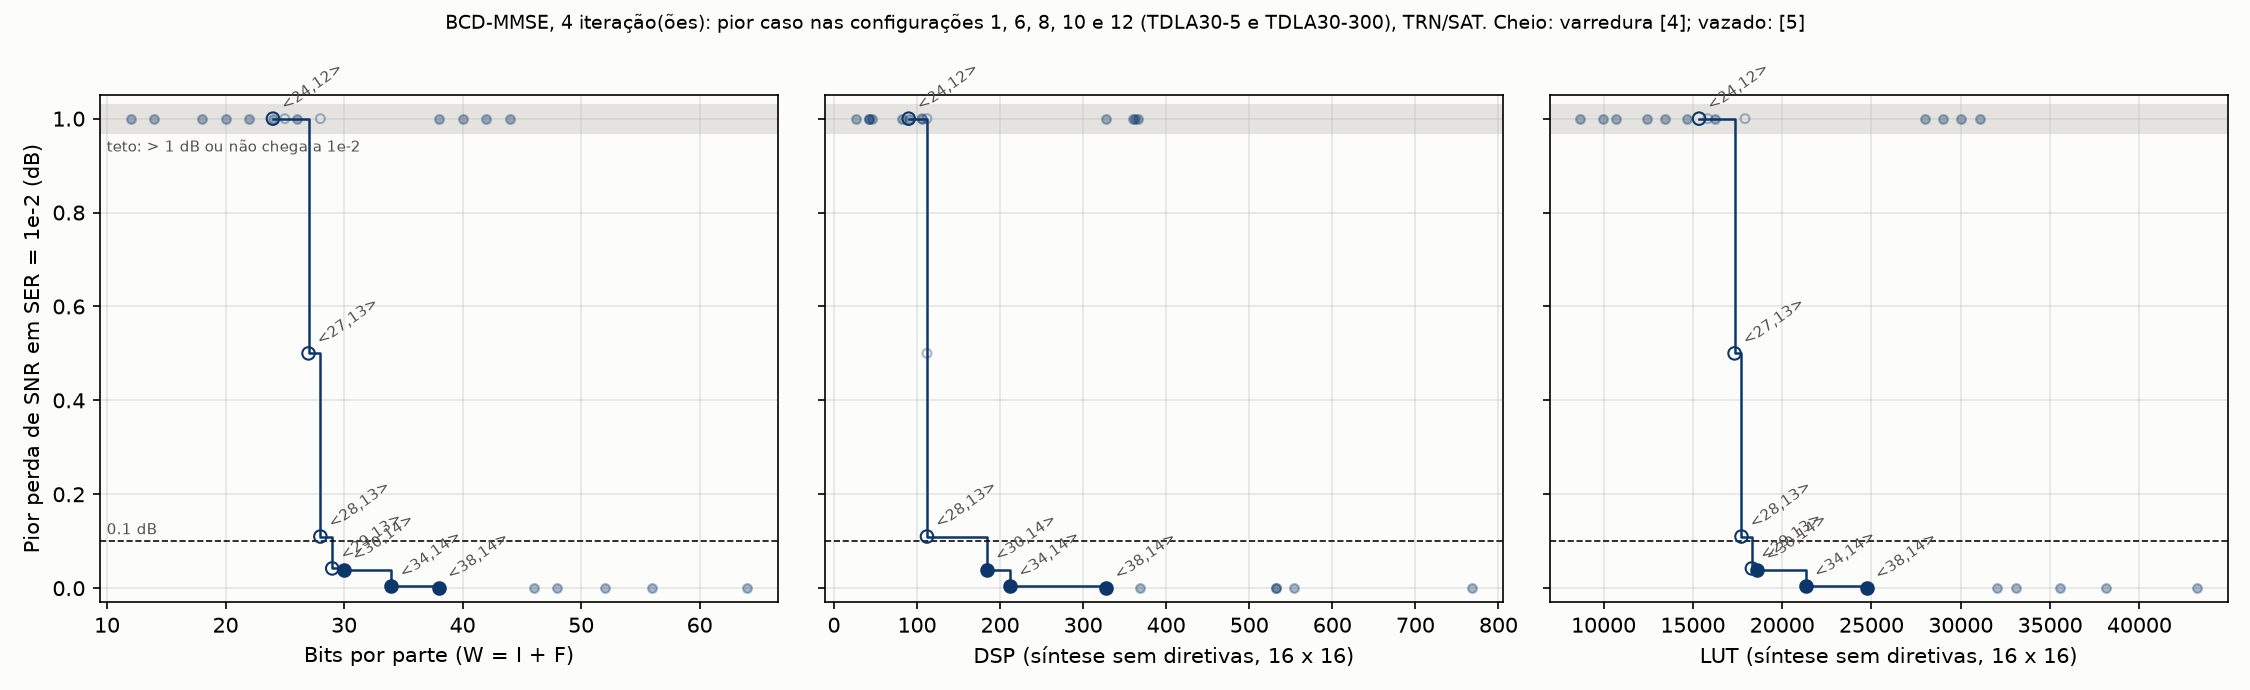
\includegraphics[width=\linewidth]{../../../software/testes/resultados/pareto/pareto_iter4.png}
\end{center}
\novo{Fronteira com 4 iterações. Cheio: formatos da [4]; vazado: da [5]. A linha tracejada é o
limiar de 0,1~dB; no teto ficam os formatos que perdem mais de 1~dB ou não chegam a $10^{-2}$.}

\novo{Lendo a fronteira:}
\begin{itemize}
  \item \novo{\textbf{Os DSP sobem em degraus.} Formatos com o mesmo $W$ usaram os mesmos DSP
        (\texttt{<24,12>} e \texttt{<24,14>}: 90; \texttt{<28,12>} e \texttt{<28,13>}: 112).
        De $W = 28$ para $W = 29$, o número salta de 112 para 184 (64\% a mais). Os LUT sobem
        quase em linha reta.}
  \item \novo{\textbf{Até 3 iterações}: \texttt{<28,13>} (112 DSP) é o mais barato abaixo de 0,1~dB.
        Ele custa o mesmo que \texttt{<27,13>} e perde menos.}
  \item \novo{\textbf{Com 4 iterações}: \texttt{<28,13>} perde 0,11~dB. É preciso subir para o degrau
        de 184 DSP, com \texttt{<29,13>} ou \texttt{<30,14>}. Os dois custam quase o mesmo, e
        \texttt{<30,14>} tem o dobro da faixa.}
  \item \novo{\textbf{O bit inteiro de folga custa um degrau com 15 bits fracionários.}
        \texttt{<29,14>} teria $W = 29$, então deve cair no degrau de 184 DSP, como o
        \texttt{<29,13>}. Isso é uma dedução: \texttt{<29,14>} não foi sintetizado nem simulado.}
\end{itemize}
\novo{Ressalvas: o custo é o da versão sem diretivas, e os degraus podem mudar com elas; as perdas de
\texttt{<27,13>}, \texttt{<28,13>} e \texttt{<29,13>} vêm de outra rodada (a [5], com a grade
inteira de SNR e outros sorteios); e \texttt{<28,13>} com 4 iterações fica muito perto do limiar
(0,11~dB).}

\subsection*{Configurações}

Os parâmetros do sistema que mudam entre as simulações. As configurações 1, 2, 3, 5, 9 e 13
são as do artigo base (Zhao et al., Fig.~8); as outras cruzam $K = 12$ e IoT de 20~dB com as
outras bases. A numeração segue $(M, C)$; com $M = 128$, primeiro 16-QAM e depois QPSK; dentro de
cada grupo, $K$ e depois a IoT.
\[
  M_c = M / C \quad \text{(antenas por \textit{cluster})}, \qquad r = 8 \text{ interferentes em todas.}
\]

\begin{center}
\small
\renewcommand{\arraystretch}{1.15}
\begin{tabular}{|c|c|c|c|c|c|c|l|}
\hline
Configuração & $M$ & $C$ & $M_c$ & $K$ & IoT (dB) & Modulação & Observação \\
\hline
1  & 128 & 8  & 16 & 8  & 10 & 16-QAM & referência do artigo\novo{; caso típico da [4]} \\
2  & 128 & 8  & 16 & 8  & 20 & 16-QAM & do artigo \\
3  & 128 & 8  & 16 & 12 & 10 & 16-QAM & do artigo \\
4  & 128 & 8  & 16 & 12 & 20 & 16-QAM &  \\
\hline
5  & 128 & 8  & 16 & 8  & 10 & QPSK   & do artigo; mesma matriz da 1 \\
6  & 128 & 8  & 16 & 8  & 20 & QPSK   & mesma matriz da 2; pior caso \novo{da [4] e} dos candidatos, com a 8 \\
7  & 128 & 8  & 16 & 12 & 10 & QPSK   & mesma matriz da 3 \\
8  & 128 & 8  & 16 & 12 & 20 & QPSK   & mesma matriz da 4\novo{; caso extremo da [4]} \\
\hline
9  & 256 & 8  & 32 & 8  & 10 & 16-QAM & do artigo \\
10 & 256 & 8  & 32 & 8  & 20 & 16-QAM & \novo{caso extremo da [4] ($M_c = 32$)} \\
11 & 256 & 8  & 32 & 12 & 10 & 16-QAM & \velho{extremo de precisão pelas métricas da matriz} \\
12 & 256 & 8  & 32 & 12 & 20 & 16-QAM & \novo{caso extremo da [4] ($M_c = 32$)} \\
\hline
13 & 256 & 16 & 16 & 8  & 10 & 16-QAM & do artigo \\
14 & 256 & 16 & 16 & 8  & 20 & 16-QAM &  \\
15 & 256 & 16 & 16 & 12 & 10 & 16-QAM &  \\
16 & 256 & 16 & 16 & 12 & 20 & 16-QAM &  \\
\hline
\end{tabular}
\end{center}

$M$: antenas da estação base; $C$: número de \textit{clusters} (DUs); $K$: usuários atendidos;
IoT: interferência sobre o ruído térmico.

\subsection*{Por que nem todas as configurações estão em [2] e em [4]}

\paragraph{Amostra [2]: sem as configurações 5 a 8.} O hardware inverte
$\mathbf G_c = E_s \mathbf H_c \mathbf H_c^H + \hat{\mathbf R}_{cc}$, que depende só do canal,
do ruído e de $E_s$: os símbolos transmitidos, e portanto a modulação, não entram nela. As
configurações 5 a 8 são iguais às 1 a 4, só que com QPSK em vez de 16-QAM. Com
a mesma semente, usam os mesmos canais e as mesmas amostras de ruído, e o hardware recebe as
mesmas matrizes. Amostrá-las só repetiria matrizes que já estão na amostra.

\paragraph{Varredura [4]: \novo{as configurações 1, 6, 8, 10 e 12}.} Com as 16 configurações e os 5 pares,
os $19 \times 35 = 665$ formatos e modos dariam cerca de 53 mil rodadas, ou semanas de
simulação. \novo{A varredura ficou com 5 configurações e 2 pares, escolhidos pela métrica do
ponto de operação (próxima seção): as configurações 6 e 8 (QPSK, IoT de 20~dB), que ficam no
topo da lista; as 10 e 12 (16-QAM, $M_c = 32$), porque a métrica falha com $M_c = 32$; e a 1,
como caso típico. Os pares são os de maior perda, (192; 3,5~GHz) e (168; 28~GHz). Com só 4 SNRs
por caso, foram 6.650 rodadas em cerca de 7 horas.}

\subsection*{\novo{Como os casos extremos da [4] foram escolhidos}}

\novo{Uma primeira ideia seria escolher pelas métricas das matrizes em todas as SNRs da grade:
maior valor, número de condição, maior valor da inversa. Elas apontam as configurações 11 e 12
($M_c = 32$), que têm o maior número de condição e os maiores valores ao longo da grade. Mas a
perda é medida só no ponto de operação, e a modulação muda onde ele fica. A matriz da
configuração 6 é a mesma da 2, mas, com QPSK, a curva chega a SER $= 10^{-2}$ perto de
$-10$~dB, justamente onde as matrizes têm os maiores valores. Com 16-QAM, essa região fica com
SER entre 0,5 e 0,9, e não pesa na medida em $10^{-2}$. Ou seja: a modulação não muda a matriz,
mas muda quais matrizes pesam no resultado. Por isso a métrica} olha só as matrizes \novo{do
ponto de operação}. Ela não precisa de nenhuma simulação
nova: usa a referência [1] e as métricas das 140.800 matrizes de cada par, que já estão
calculadas.
\begin{enumerate}
  \item Pela referência [1], achar o ponto de operação de cada configuração e par (aqui, com 1
        iteração).
  \item Pegar todas as matrizes $\mathbf G_c$ dos dois pontos da grade em volta dele. Por
        exemplo, se a curva cruza em $-9{,}3$~dB, as de $-10$ e $-8$~dB. As configurações 5 a 8
        usam as matrizes das 1 a 4, porque a modulação não muda $\mathbf G_c$.
  \item Em cada matriz, anotar o maior valor: a maior parte real ou imaginária, em módulo.
  \item Desses valores, pegar o percentil 99, o valor que só 1\% das matrizes ultrapassa. O
        máximo absoluto não é usado porque pode vir de uma única matriz rara, que quase não muda a
        SER.
  \item Os casos com esse número mais alto são os extremos. Se ele passa do limite do formato
        ($\pm 2048$ com $I = 12$, $\pm 4096$ com $I = 13$), o formato satura.
\end{enumerate}

\begin{center}
\small
\renewcommand{\arraystretch}{1.15}
\begin{tabular}{|c|c|c|c|c|c|}
\hline
Config. & Par $(N, f_c)$ & Ponto de operação & $\mathbf G_c$ (percentil 99) & Perda \texttt{<28,12>} & Perda \texttt{<25,13>} \\
\hline
8  & 192; 3,5~GHz & $-8{,}7$~dB & 2.470 & 0,32 & 1,35 \\
8  & 132; 3,5~GHz & $-8{,}6$~dB & 2.402 & 0,33 & 1,48 \\
6  & 192; 28~GHz  & $-9{,}2$~dB & 2.387 & 0,58 & 1,72 \\
6  & 168; 28~GHz  & $-9{,}1$~dB & 2.383 & 0,58 & 1,76 \\
6  & 192; 3,5~GHz & $-9{,}3$~dB & 2.266 & 0,60 & 1,63 \\
\hline
8  & 24; 3,5~GHz  & $-6{,}5$~dB & 1.646 & 0,00 & 1,06 \\
6  & 24; 3,5~GHz  & $-7{,}2$~dB & 1.428 & 0,00 & 1,29 \\
\hline
10 & 192; 28~GHz  & $-5{,}8$~dB & 998   & 0,00 & 1,69 \\
12 & 168; 28~GHz  & $-5{,}5$~dB & 987   & 0,01 & 1,51 \\
\hline
\end{tabular}
\end{center}
Perdas em dB, com AP\_TRN e 1 iteração, medidas nos candidatos [5]. \texttt{<28,12>} mostra a
saturação ($I = 12$); \texttt{<25,13>}, a falta de precisão ($F = 12$). A tabela mostra só alguns
dos 80 casos: os do topo, os do par com $N = 24$ e os com $M_c = 32$.

\paragraph{O que a métrica acerta.}
\begin{itemize}
  \item \textbf{Os piores casos.} Os 8 primeiros dos 80 casos são as configurações 6 e 8 com
        $N \ge 132$, justamente o pior caso dos candidatos.
  \item \textbf{O limite de $I$.} Em todos os casos com o número acima de 2.048, $I = 12$ perdeu
        de 0,28 a 0,60~dB. Abaixo disso, perdeu no máximo 0,01~dB, inclusive com $N = 24$. A métrica
        diz, antes de rodar o hardware, se um $I$ basta.
  \item \textbf{A ordem da precisão.} Quanto maior $\mathbf G_c$, menores os valores da inversa,
        e mais o truncamento pesa. Ordenando os 80 casos pela métrica e pela perda de
        \texttt{<25,13>}, as duas listas ficam quase na mesma ordem (correlação de postos de
        Spearman de 0,93). O número de condição no ponto de operação deu só 0,68.
\end{itemize}

\paragraph{Onde ela falha.} As configurações 10 e 12 ($M_c = 32$) têm $\mathbf G_c$ com cerca de
1.000, metade das 6 e 8, e mesmo assim perdem quase o mesmo em precisão (1,5 a 1,7~dB). Uma
explicação provável, não testada à parte: a matriz $32 \times 32$ faz mais contas, e os erros de
truncamento se acumulam. Por isso a escolha deve incluir uma configuração com $M_c = 32$, mesmo
que ela não esteja no topo da lista.

\paragraph{\novo{A escolha.}} Configurações 6 e 8 (QPSK, IoT de 20~dB), mais uma
com $M_c = 32$ (10 ou 12, que dão quase o mesmo resultado); pares $(192; 3{,}5~\text{GHz})$ e
$(168; 28~\text{GHz})$, os de maior perda. O par com $N = 24$ é o mais fácil
nos dois eixos: com $N = 24$, a curva cruza $10^{-2}$ numa SNR mais alta, onde $\mathbf G_c$ é
menor. Essa escolha foi conferida com os resultados da [5]; a métrica em si não precisa deles.

\novo{\textbf{O resultado na [4].} A [4] usou essa escolha, com a configuração 1 como caso
típico e as duas com $M_c = 32$. Os piores casos da [4] foram as configurações 6 e 8, como a
métrica previa, e os menores formatos da grade ($I = 14$, $F = 16$) ficaram iguais ao limite
da [5].}

\subsection*{Pares $(N, f_c)$}

Cada condição de teste da norma (TS 38.104, Anexo G) define duas coisas para o simulador:
o número $N$ de amostras de ruído por PRB, que vem do tempo de coerência e do DM-RS, e a
frequência da portadora $f_c$. Condições com o mesmo par dão o mesmo resultado, então cada
par foi simulado uma vez.

A portadora muda o resultado porque, no cenário UMa NLOS do QuaDRiGa, o espalhamento angular
depende da frequência (cerca de 86° de espalhamento de chegada a 3,5~GHz e 49° a 28~GHz), e
isso muda a correlação entre as antenas. A velocidade só entra pelo tempo de coerência, ou seja,
pelo $N$: o canal é considerado constante dentro do bloco de coerência, sem Doppler.

\begin{center}
\small
\renewcommand{\arraystretch}{1.15}
\begin{tabular}{|c|c|c|l|l|}
\hline
Par & $N$ & $f_c$ & Condições de teste & Mobilidade típica \\
\hline
1 & 192 & 3,5~GHz (FR1) & TDLA30-5, TDLA30-10 & baixa \\
2 & 192 & 28~GHz (FR2)  & TDLA30-75           & baixa \\
3 & 168 & 28~GHz (FR2)  & TDLA30-300          & média a alta \\
4 & 132 & 3,5~GHz (FR1) & TDLC300-100         & média a alta \\
5 & 24  & 3,5~GHz (FR1) & TDLB100-400         & média a alta \\
\hline
\end{tabular}
\end{center}

As condições HST350 e HST500 (trem de alta velocidade) ficaram de fora: o tempo de coerência
dura um símbolo OFDM, e a maioria dos símbolos de dados não tem nenhuma amostra de ruído
($N = 0$).

\end{document}
